\section{Mikrofon}
Til at måle lydinputs til systemet, er der valgt en electret condensator mikrofon fra Adafruit \cite{manual_mic}, med tilhørende for-forstærker \cite{manual_amp}. 
Mikrofonen er designet til at arbejde sammen med Arduino, og har et DC-offset på halvdelen af forsyningspændingen, hvilket gør det nemt at skifte reference. 
Desuden er mikrofonen egnet til optagelse i området $20 Hz - 20 kHz$, hvilket passer fint til projektet. 
Gain-indstillingen på mikrofon-kittet kan bruges til at kalibrere systemet mht. korrekt måling af lydtryksniveau. 

\subsection{Sampling af lydinput}
Samplingen af lydsignalet sker gennem Arduinoens ADC. 
Ved sampling af lydsignaler er der to essentielle parametre, som skal bestemmes.
Den ene parameter er samplefrekvens. 
Samplefrekvensen sætter en øvre grænse for, hvor højt frekvensindhold, systemet kan måle. 
Som udgangspunkt skal samplefrekvensen være så høj som muligt, og for at kunne måle indenfor hele det hørbare spektrum kræves en samplefrekvens på mindst $40 kHz$. 
Den anden parameter er bit-dybden.
Bit-dybden bestemmer opløsningen for optagelsen, og dermed, hvor stor en dynamisk spændevidde systemet vil kunne fange. 
Bit-dybden for audio er typisk 16-24 bit. 
Begge parametre stiller krav til systemet, mht. hastighed og hukommelse. 

Arduinoens ADC har en maksimal bit-dybde på 10 bit, hvilket resulterer i en dynamisk spændevidde på $ 20 \cdot \log (2^{10}) = 60 dB$. 
Ved 10 bit opløsning er ADC'ens clock dog begrænset til $200 kHz$. 
Én konvertering tager $13.5$ clock cycles, og samplefrekvensen kan maksimalt blive $ 15 kHz$.
Det resulterer i en Nyquist-frekvens på $7.5 kHz$, hvilket er temmelig lavt ift. det fulde spektrum. 
Hvis bit-dybden reduceres til 8 bit, kan ADC'ens clock-frekvens hæves op til $1 MHz$. 
På den måde er samplefrekvensen ikke en begrænsning. 
Dog giver en 8 bit opløsning kun et signal-støjforhold på $48 dB$. 

Som et kompromis er der valgt en 8 bits opløsning og en samplefrekvens på $20 kHz$.
Begrundelsen for den lave samplefrekvens forklares under afnittet om frekvensanalyse. 

\subsection{Antialiasering}
For at undgå aliasering og indstråling af højfrekvent støj, skal mikrofonens output filtreres gennem et anti-aliaseringsfilter.
Filteret er et anden ordens RLC-lavpasfilter, og er realiseret med en knækfrekvens på Nyquist-frekvensen. 
Filteret kunne med fordel laves skarpere end et anden ordens filter, men i første omgang er proof of concept mere væsentligt end ydeevne. 
Verifikation og test af filteret kan ses i afsnittet om modultests og integrationstests.

\begin{figure}[H]
	\center
	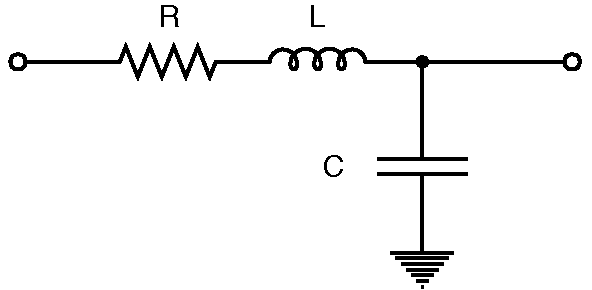
\includegraphics[width=0.3\textwidth]{Figur/RCL_diagram.pdf}
	\caption{RCL-lavpasfilter}
	\label{fig:RCL}
\end{figure}

\subsection{Konfiguration}
Konverteringen af det analoge data sker i ADC 0 i single ended mode med $5 V$ reference fra AREF. 
AREF kunne med fordel forbindes til en mere stabil forsyning, end $5 V$ men det shield, som skærmen sidder på, besværliggør dette. 
Konverteringen sættes til automatisk start på interrupt. 
Interruptet vælges til at komme fra Timer 1 på compare B-interruptet jf. databladet \cite{manual_arduino}.

ADC'en aktiveres ikke i første omgang. 
I stedet aktiveres den når \textit{record()}-funktionen kaldes. 
Første sample efter aktiveringen bliver derfor beskadiget.
Principielt burde samplet kasseres, men da hele optagelsen bliver foldet med et Hanning-vindue, har det ingen betydning. 

Til at styre samplefrekvensen, bruges timer 1 i CTC mode. 
OCR-værdien regnes ved: $$ OCR = \frac{F_{CPU}}{2 \cdot K \cdot F_s - 1}, $$ hvor $K$ er prescaler-værdien.
OCR rundes af til $399 $ uden prescaling, for en frekvens på $20 kHz$. 

For at \textit{color} kan tilgå data i \textit{fht\_log\_out}, har \textit{mic} en \textit{getFHTptr()}-metode, som giver den en pointer til arrayet. 

\section{Frekvensanalyse}
Til at analysere på det optagede signal, bruges en diskret Hartley Transformation, forkortet FHT. 
FHT er en afart af diskret Fourier transformation, designet specifikt til reel data. 
Algoritmen til at udføre FHT er fundet ved Open Music Labs, som er et audio-forum under Flingco Sound System. \cite{fht_arduino}

\subsection{Kvalitet af analyse}
Transformationen har i denne algoritme en maksimal længde på 256 samples, hvilket giver en frekvensopløsning på: $$ \Delta f = \frac{20 kHz}{256 samples} = 78.125 Hz$$ 
En samplefrekvens på $ 40 kHz$ ville have dobbelt så store frekvens-bins, hvilket ville gøre det svært at skelne frekvensinholdet i de laveste frekvenser. 
Derfor er begrænsningen på $20 kHz $ sat. 

En længere FHT er selvfølgelig mulig, men da dette projekt, udelukkende med mikrofon, FHT og skærm, fylder $17 \%$ af datahukommelsen, vil det sandsynligvis ikke kunne lade sig gøre. 
Zero-padding er også en mulighed for at forbedre frekvensopløsningnen, men så skulle halvdelen af algoritmens look-up tabeller alligevel forstørres. 
